\section{Barbalat 引理}

\begin{frame}
  \frametitle{Barbalat 引理}
  \framesubtitle{函数及其导数的渐进性质}
  $\dot{f}\to 0 $
  $\nRightarrow$
  $f$ 收敛

  函数的倒数趋于零$\dot{f}\to 0 $并不等价于函数收敛$\exists C\in\mathbb{R},\lim_{t\to\infty}f(t)=C$.

  \begin{block}{example}
    \begin{enumerate}
      \item 有界函数:$f_1(t)=\sin(\ln t)$,$\dot{f}_1(t)=\frac{\cos(\ln t)}{t}$
      \item 无界函数:$f_2(t)=\sqrt{t} \sin(\ln t)$,$\dot{f}_2(t)=\frac{\sin(\ln t)}{2 \sqrt{t}}+ \frac{\cos (\ln t)}{\sqrt{t}}$
    \end{enumerate}

    这两个函数的导数都趋于零,但是函数不收敛.

    \begin{figure}
      \centering
      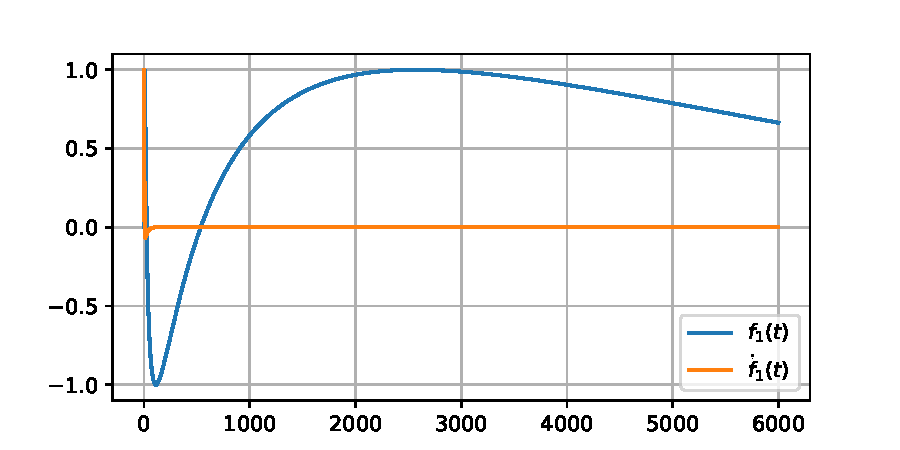
\includegraphics[height=2.8cm]{figure/sinlnt.pdf}
      \quad
      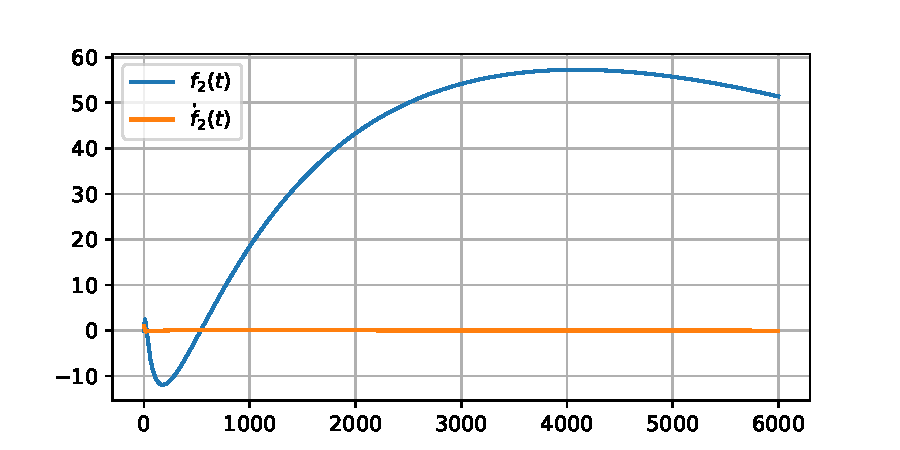
\includegraphics[height=2.8cm]{figure/sqrttsinlnt.pdf}
    \end{figure}
  \end{block}
\end{frame}

\begin{frame}
  \frametitle{Barbalat 引理}
  \framesubtitle{函数及其导数的渐进性质}

  $f$ 收敛
  $\nRightarrow$
  $\dot{f}\to 0 $

  函数收敛并不意味着函数倒数趋于零$\dot{f}\to 0$.

  \begin{block}{Tip: 与Lyapunov的联系}
    这个现象说明:
    如果一个函数$f$有下界并且为非增函数$\dot{f}\leq 0$,
    那么这个函数收敛到一个极限。
    \textbf{但是这个函数的导数不一定收敛到零}
  \end{block}

  \begin{block}{Example 1}
    另一个例子是周期脉冲信号:

    \begin{figure}
      \centering
      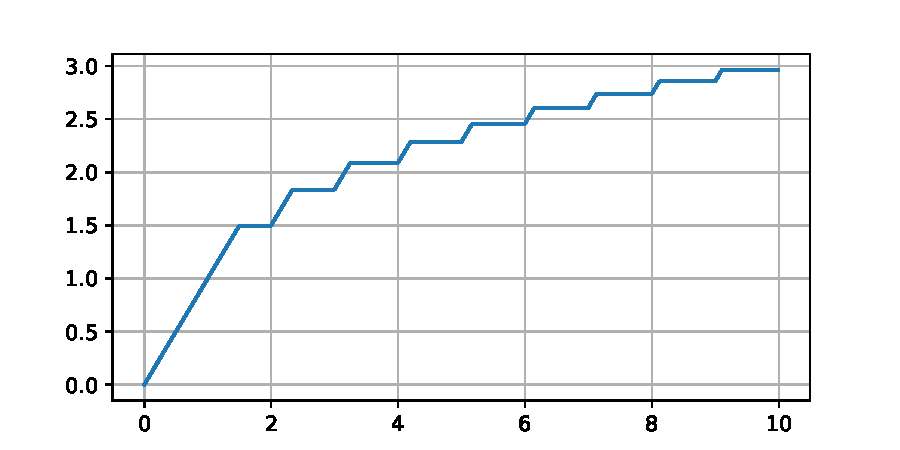
\includegraphics[height=2.6cm]{figure/barbalat_f4.pdf}
      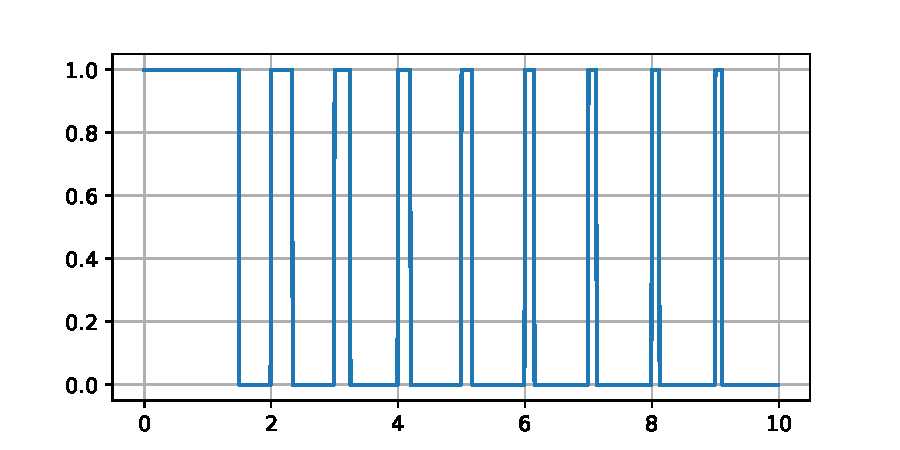
\includegraphics[height=2.6cm]{figure/barbalat_f4d.pdf}
    \end{figure}
  \end{block}
\end{frame}


\begin{frame}
  \begin{block}{Example 2}
    $f(t)=e^{-t}\sin (e^{2t})$收敛到零,但是其导数
    \[
      \dot{f}=-e^{-t}\sin(e^{2t}) + 2 e^{t} \cos(e^{2t})
    \]
    是一个有界函数。

    \begin{figure}
      \centering
      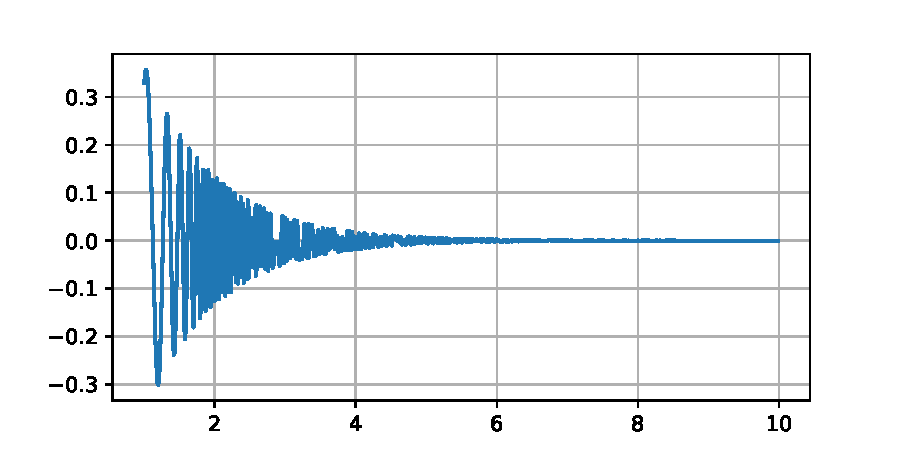
\includegraphics[height=2.6cm]{figure/barbalat_f3.pdf}
      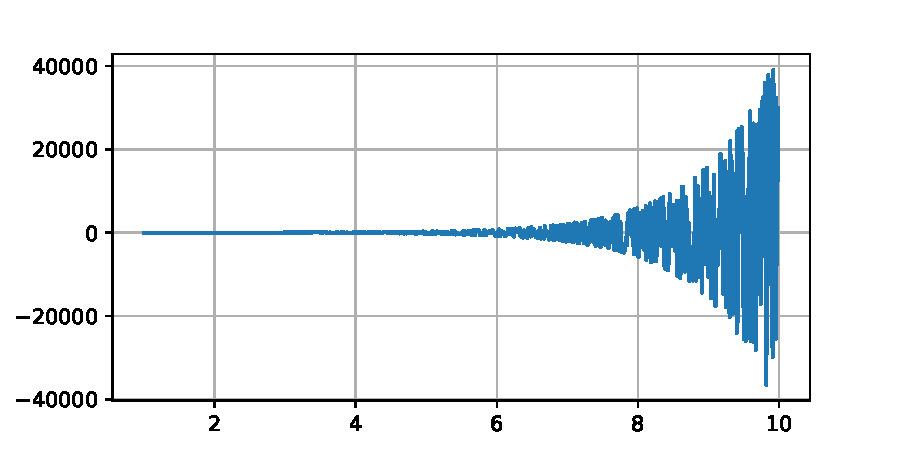
\includegraphics[height=2.6cm]{figure/barbalat_f3d.pdf}
    \end{figure}
  \end{block}
\end{frame}

\begin{frame}
  \frametitle{Barbalat‘s 引理的基本形式}

  \begin{lemma}
  设 $x:[0, \infty) \to \mathbb{R}$ 为一阶连续可导,且当 $t \to \infty$ 时有极限,则如果 $\dot{x}(t), t \in [0, \infty)$ 一致连续,那么 $\lim\limits_{t \to \infty} \dot{x}(t) = 0$。
  \end{lemma} 

  如果 $\ddot{x}(t)$ 存在且有界,那么引理1中 $\dot{x}(t)$ 的一致连续性条件可用 $\ddot{x}(t)$ 的有界性来替代,从而得到如下形式的引理。

  \begin{lemma}
  设 $x:[0, \infty) \to \mathbb{R}$ 一阶连续可导,且当 $t \to \infty$ 时有极限,则如果 $\ddot{x}(t), t \in [0, \infty)$ 存在且有界,那么 $\lim\limits_{t \to \infty} \dot{x}(t) = 0$。
  \end{lemma}

  如下推论是显而易见的。

  \begin{corollary}
    若 $x: [0, \infty) \to \mathbb{R}$ 一致连续,并且 $\lim\limits_{t \to \infty} \int_{0}^{t} x(\tau) \mathrm{d}\tau$ 存在且有界,那么 $\lim\limits_{t \to \infty} x(t) = 0$。
  \end{corollary}
\end{frame}

\begin{frame}
  \frametitle{回顾不变集原理}
  考虑自治系统
\[
\dot{x} = f(x) \tag{1}
\]
其中 $x \in \mathbb{R}^n$,$f: D \to \mathbb{R}^n$ 是局部 Lipschitz 函数,$D \subseteq \mathbb{R}^n$ 为定义域。

  设 $V: D \to \mathbb{R}$ 是连续可微函数,且满足:
  \begin{enumerate}
      \item 存在 $c \geq 0$,使得集合 $S = \{x \in D \mid V(x) \leq c\}$ 是有界的,且 $S \subseteq D$;
      \item 对所有 $x \in S$,有 $\dot{V}(x) \leq 0$,其中 $\dot{V}(x) = \nabla V(x) \cdot f(x)$ 是 $V$ 沿系统(1)轨迹的导数。
  \end{enumerate}

  定义集合
  \[
  E = \{x \in S \mid \dot{V}(x) = 0\}
  \]
  并设 $M$ 是 $E$ 中最大的不变集(相对于系统(1)而言)。则系统(1)的每一条解轨迹 $x(t)$ 均有界,且当 $t \to \infty$ 时收敛到 $M$。


  若在上述定理中,最大不变集 $M$ 仅包含平衡点 $x = 0$,即 $M = \{0\}$,则该平衡点是渐近稳定的。进一步,若 $D = \mathbb{R}^n$ 且当 $\|x\| \to \infty$ 时 $V(x) \to \infty$,则该平衡点是全局渐近稳定的。
\end{frame}


\begin{frame}
  \frametitle{Barbalat's 引理在李亚普诺夫分析中的应用}

  考虑非自治系统
\[
\dot{x} = f(t,x) 
\]
其中 $x \in \mathbb{R}^n$,$f: D\times[0,\infty) \to \mathbb{R}^n$ 是局部 Lipschitz 函数,$D \subseteq \mathbb{R}^n$ 为定义域。
  
  \begin{theorem}
    如果一个标量函数$V(t,x)$ 满足如下条件:
    \begin{enumerate}
      \item $V(t,x)$ 有下界;
      \item $\dot{V}(t,x)$ 是半负定;
      \item $\dot{V}(t,x)$ 关于时间是一致连续的
    \end{enumerate}
    那么 有$\lim_{t\to\infty} \dot{V}(t,x)=0$
  \end{theorem} 
\end{frame}